

\subsection{Panels}

\begin{table}[h!]\footnotesize
\begin{tabularx}{\textwidth}{lc}
\rowcolor{Gray}
Flurochrome  & \\
Alexa-488    & CD127\\
PE-Cy7       & HLADR\\
APC          & CD25\\
PE           & CD101\\
Alexa-700    & CD4\\
Pacific Blue & CD45RA\\
\end{tabularx}
\caption{ \label{IL2RA-panels}
The fluorochrome-antibody panels with six markers used in the ILRA dataset.
}
\end{table}



%\begin{table}
%\begin{center}
%\begin{tabular} {|c | c |}
%\cline{1-2}
%Fluorochrome & Antibody Target\\
%\cline{1-2}
%APC & CD25 \\
%Pacific Blue & CD45RA \\
%Alexa 488 & CD127 \\
%Alexa 700 & CD4 \\
%%PE & FOXP3 \\
%\cline{1-2}
%\end{tabular}
%\end{center}
%\caption{ Subset of the fluorochrome-antibody panel used by \citet{Dendrou:2009dv} to identify non T regs in whole blood. }
%\label{table:panel} 
%\end{table}
%


%CD101,CD127,CD25_MA251+2A3,CD4,CD45RA,HLADR
%CD127,CD25_MA251+2A3,CD4,CD45RA,ISO 

\subsection{Samples}

A total of 224 FCS files.


The experiment consisted of a total of $219$ individuals

$180$ from unique individuals $16$ of which were recalled for a second sample.


Individuals were selected based on the three SNPs and split into to seven genotype groups.
Within each group there are about as many males as females and with similar age distribution across all groups ($20$ to $50$ years old).
The running time of the whole experiment was seven months over which samples were analysed on $51$ days (between one and six samples on each day).



\begin{figure}
\centering
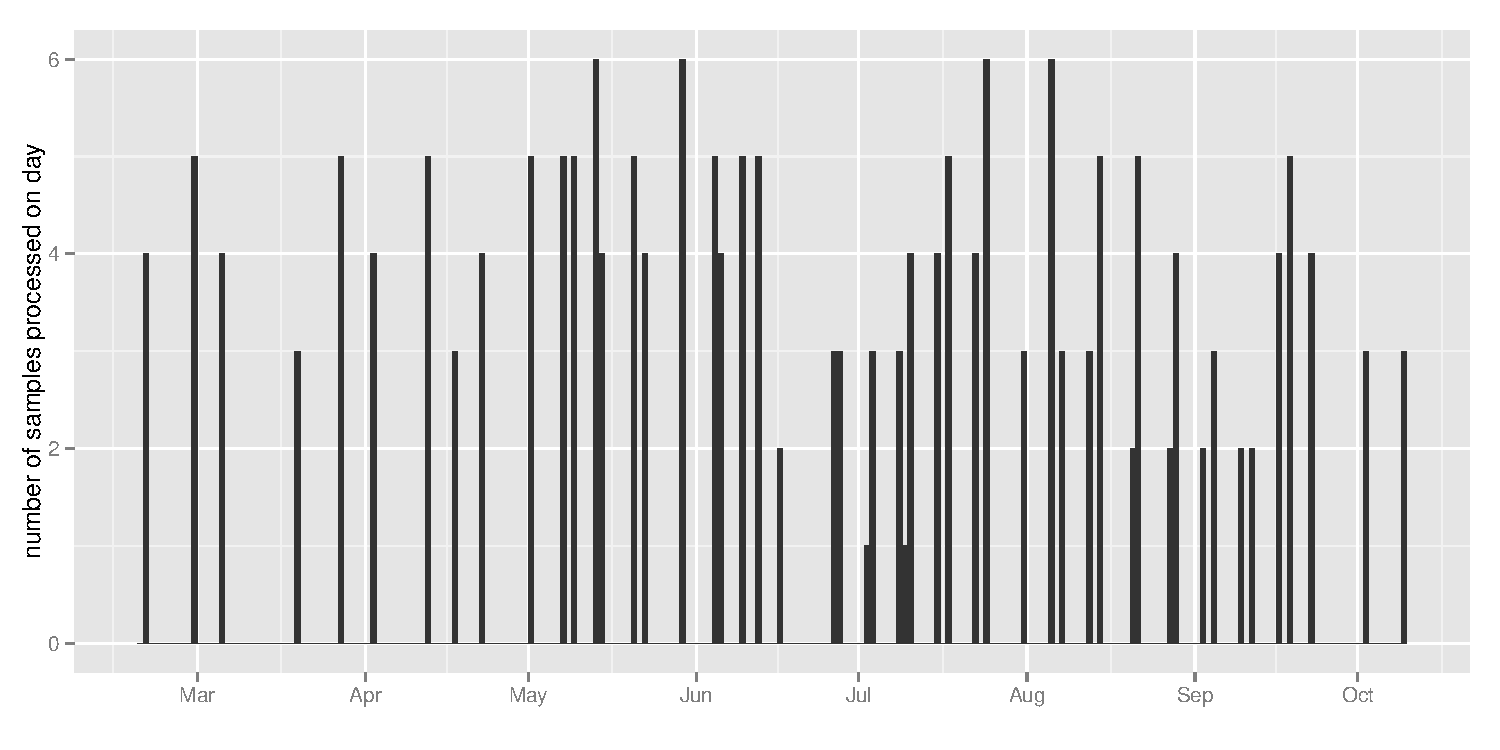
\includegraphics[scale=.5] {flowdatasets/figures/il2ra-samples-time.pdf}
\caption{
\label{figure:IL2RA-sample-time} 
}
\end{figure}


\begin{table}[ht]
\centering
\begin{tabular}{lllllll}
  \hline
         & individual & pch & day1       & day2       & day diff \\
  \hline
  1      & CB00058M   & a   & 2008-03-04 & 2008-09-16 & 196 \\
  2      & CB00427N   & b   & 2008-02-20 & 2008-10-02 & 225 \\
  3      & CB00435X   & c   & 2008-02-28 & 2008-10-02 & 217 \\
  4      & CB00459Y   & d   & 2008-03-26 & 2008-10-09 & 197 \\
  5      & CB00470K   & e   & 2008-04-10 & 2008-09-18 & 161 \\
  6      & CB00474P   & f   & 2008-04-16 & 2008-09-16 & 153 \\
  7      & CB00475Q   & g   & 2008-05-08 & 2008-09-18 & 133 \\
  8      & CB00496N   & h   & 2008-05-12 & 2008-09-22 & 133 \\
  9      & CB00503W   & i   & 2008-05-06 & 2008-09-18 & 135 \\
  10     & CB00555C   & j   & 2008-05-22 & 2008-09-16 & 117 \\
  11     & CB00563L   & k   & 2008-05-29 & 2008-09-18 & 112 \\
  12     & CB00566P   & l   & 2008-05-29 & 2008-09-18 & 112 \\
  13     & CB00568R   & m   & 2008-05-29 & 2008-09-22 & 116 \\
  14     & CB00588N   & n   & 2008-06-12 & 2008-10-09 & 119 \\
  15     & CB00591R   & o   & 2008-06-16 & 2008-09-22 & 98 \\
  16     & CB00646B   & p   & 2008-07-15 & 2008-10-02 & 79  \\
  \hline
\end{tabular}
\caption{ \label{table:IL2RA-recalled-individuals} Sixteen individuals recalled between 79 and 226 days later. }
\end{table}




\subsection{Manual Gating}





